\chapter{Исследовательская часть}

\section{Технические характеристики}
Тестирование выполнялось на устройстве со следующими техническими характеристиками:
\begin{itemize}
	\item Операционная система Pop!\_OS 22.04 LTS \cite{ubuntu} Linux \cite{linux};
	\item Оперативная память 16 Гб;
	\item Процессор AMD® Ryzen 7 2700 eight-core processor × 16 \cite{amd}.
\end{itemize}
Во время тестирования устройство было подключено к блоку питания и не нагружено никакими приложениями, кроме встроенных приложений окружения, окружением и системой тестирования.

\section{Сравнение с реальным преломлением}

При одинаковом коэффициенте преломления равным 1 у цилиндра и жидкости, стержень не должен иметь преломление, то есть не должно быть ступенек при переходе между средами.

На рисунке \ref{img:inter-coef-1} продемонстрировано, что коэффициенты жидкости и цилиндра равны. 

\begin{figure}[ht!]
	\centering{
		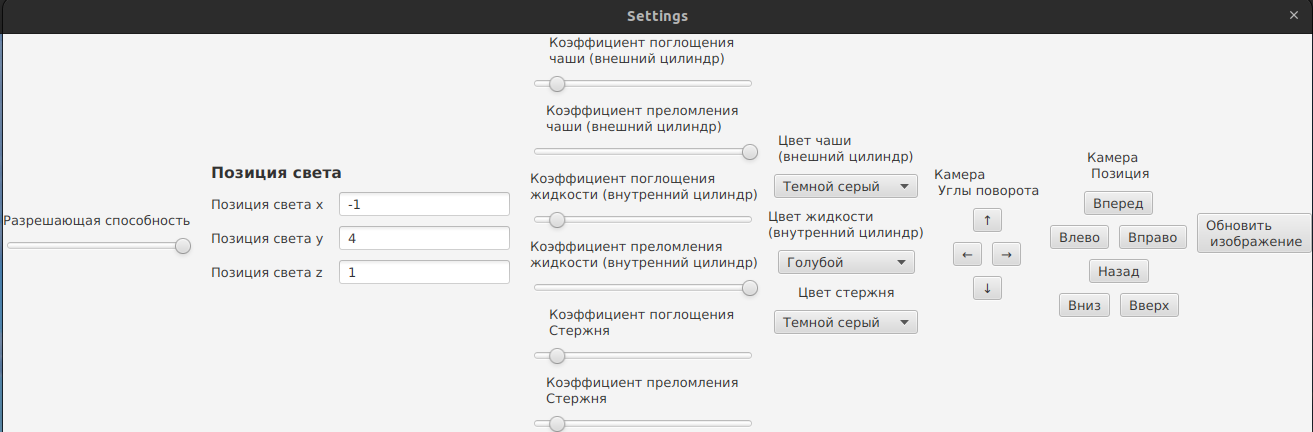
\includegraphics[width=0.8\textwidth]{assets/coef-1.png}
		\caption{Интерфейс программы}
		\label{img:inter-coef-1}}
\end{figure}

На рисунке \ref{img:inter-coef} продемонстрировано, что стержень не имеет преломления в разных средах. 

\begin{figure}[ht!]
	\centering{
		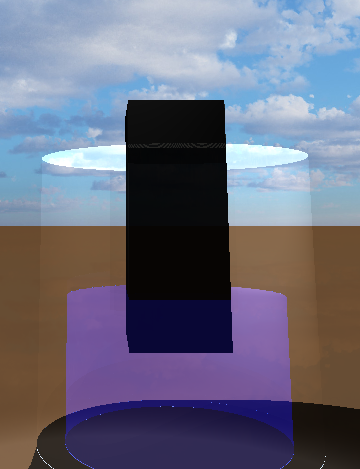
\includegraphics[width=0.4\textwidth]{assets/coef-2.png}
		\caption{Интерфейс настроек программы}
		\label{img:inter-coef}}
\end{figure}

\section{Время работы алгоритма трассировки лучей при разной глубине рекурсии}

В алгоритме обратной трассировки лучей задается глубина рекурсии.

В таблице \ref{tab:time1} продемонстрировано пользовательское время программы при разном глубине рекурсии.

\begin{table}[ht!]
	\begin{center}
		
		\caption{Пользовательское время работы программы при разной глубине рекурсии}
		\label{tab:time1}
		\begin{tabular}{|c|c|}
			\hline
			Глубина рекурсии & Время в 	нс. \\
			\hline
			1  & 779 031 434 \\
			\hline
			2  & 892 963 172 \\
			\hline
			3  & 1 282 984 014 \\
			\hline
			4  & 1 618 809 960 \\
			\hline
			5  & 2 081 470 533 \\
			\hline
			6  & 3 128 113 059 \\
			\hline
			7  & 4 830 126 723 \\
			\hline
			8  & 7 369 684 160 \\
			\hline
			9  & 12 912 481 173 \\
			\hline
			
		\end{tabular}
	\end{center}
\end{table}